\documentclass{article}
\usepackage{amsmath}
\usepackage{amsfonts}
\usepackage[a4paper]{geometry}
\usepackage{graphicx}
\usepackage{caption}
\usepackage{subcaption}
\usepackage{amsthm}

\begin{document}
\theoremstyle{plain}
\newtheorem{thm}{Theorem}
\newtheorem{lem}[thm]{Lemma}
\newtheorem{prop}[thm]{Proposition}
\newtheorem{corr}{Corollary}
\theoremstyle{definition}
\newtheorem{defn}{Definition}
\newtheorem{conj}{Conjecture}
\newtheorem{exmp}{Example}
\theoremstyle{remark}
\newtheorem*{rem}{Remark}
\newtheorem*{note}{Note}
\newtheorem{case}{Case}

\author{
Oh Shunhao\\
  \texttt{A0065475X}
  \and
Nguyen Quoc Dat\\
  \texttt{A0116703N}
}
\title{CS4234: 2D Strip Packing}
\date{}

\maketitle

\begin{abstract}
\begin{center}
The 2D Strip Packing problem is concerned with the minimum height of a fixed-width strip needed to pack a set of rectangular object into the strip. In this report, we give a brief summary of the current state-of-the art, and experiment with the practical effectiveness of some of the existing algorithms.
\end{center}
\end{abstract}

\section{Problem Definition}
In the Strip Packing problem, we are given an infinitely tall strip, of maximum width $W$, and a set of $n$ rectangular objects $s_1,s_2,\cdots,s_n$, each represented by a tuple $s_i = (w_i,h_i)$, representing the width and height of each object.\\
\\
The task is to pack all of the $n$ objects into the strip, so that none of the objects overlap, and such that the total height of the strip is minimised.\\
\\
This problem has many applications in the industry, like in manufacturing, where rectangular pieces need to be cut out of a strip of fixed width, or perhaps in sprite packing for games, where fixed-size sprites can be packed into a single image to minimise the memory footprint of a game.\\

\section{State of the Art}
The decision problem of Strip Packing easily shown to be NP-HARD via a reduction from the partition problem.\\
\\
Assuming $P \neq NP$, there is no absolute polynomial time approximation scheme for Strip Packing. In fact, there is no algorithm with an absolute approximation ratio better than $\frac{3}{2} - \epsilon$ as 1-dimensional bin-packing is a subproblem of strip packing (1-dimensional bin packing is equivalent to strip packing with objects of height $1$), and in 1-dimensional bin packing, it is NP-HARD to distinguish whether OPT is $2$ or $3$ due to a reduction from the Partition problem.\\
\\
The current best known absolute approximation algorithm has an approximation ratio of $\frac{5}{3} + \epsilon$ by Harren et. al. \cite{harren1}, which is close to the lower bound of $\frac{3}{2} - \epsilon$. On the other hand, asymptotic approximation algorithms do much better. Simple algorithms like First-Fit Decreasing Height and Split-Fit already achieve asymptotic approximation ratios of $\frac{17}{10}$ and $\frac{3}{2}$ respectively. The best known asymptotic approximation ratio for Strip Packing is $\frac{5}{4}$ by Baker et. al.  \cite{baker1}.\\

\section{Existing algorithms}
Many existing approximation algorithms for 2-D Strip Packing are level-oriented algorithms. Level-oriented algorithms involve packing items into shelves of certain heights. These algorithms include First-Fit Decreasing Height, and Split-Fit.
\subsection{First-Fit Decreasing Height}
\textit{First-Fit Decreasing Height} (FFDH) places the objects in decreasing height order one by one on the bottom of the strip. When an object cannot be placed on the bottom the strip, a new shelf is created from the top y-coordinate of the leftmost (tallest) object of the topmost shelf.\\
\\
For a given list $L$ of objects, the performance of FFDH is bounded by the following:
\[
	FFDH(L) \leq 1.7 \times OPT(L) + 1
\]
The proof for the approximation ratio of FFDH is based on the proof of the approximation ratio for the First-Fit algorithm for the one-dimensional bin packing problem, which is also asymptotically 1.7-approximate.
\subsection{Split-Fit}
\textit{Split-Fit} (SF) also sorts the objects by decreasing height. We find $m \geq 1$, which is the maximum integer such that all given objects have width less than or equal to $\frac{1}{m}$. The objects are then divided into two sets $L_1$ and $L_2$:
\begin{itemize}
\item $L_1$ contains objects with width greater than $\frac{1}{m+1}$.
\item $L_2$ contains objects with width less than or equal to $\frac{1}{m+1}$.
\end{itemize}
Then, the objects in $L_1$ are packed using FFDH. The resulting shelves produced are then rearranged by width, such that all shelves with width more than $\frac{m+1}{m+2}$ are below shelves with width less than or equal to $\frac{m+1}{m+2}$. This results in a free rectangle $R$ of width $\frac{1}{m+2}$ to the right of the shelves with width less than or equal to $\frac{m+1}{m+2}$.\\
\\
We then proceed to pack objects in $L_2$ into R, treating it as a strip of width $\frac{1}{m+2}$. However, if a new shelf is to be created, and it exceeds the height of R, then it is placed on top of the shelves from $L_1$ with width less than or equal to $\frac{m+1}{m+2}$, and thus allows the full width of the original strip. This continues until all objects have been packed.\\
\\
The performance of SF is bounded by the value of $m$:
\[
	SF(L) \leq \frac{m+2}{m+1}OPT(L) + 2
\]
In other words, if all objects have width less than or equal to one third of the strip width, then $m = 3$, and thus the performance bound for SF is $\frac{5}{4}OPT + 2$. However, in the worst case where $m = 1$ i.e. there exists at least one object with width larger than $\frac{1}{2}$, the approximation ratio for SF is:
\[
	SF(L) \leq \frac{3}{2}OPT(L) + 2
\]
\begin{figure}[ht]
\centering
\begin{subfigure}{.35\textwidth}
  \centering
  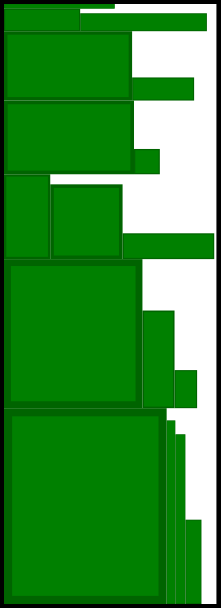
\includegraphics[width=.5\linewidth]{FFDHrun.png}
  \caption{FFDH Algorithm}
  \label{fig:ffdhrun}
\end{subfigure}%
\begin{subfigure}{.35\textwidth}
  \centering
  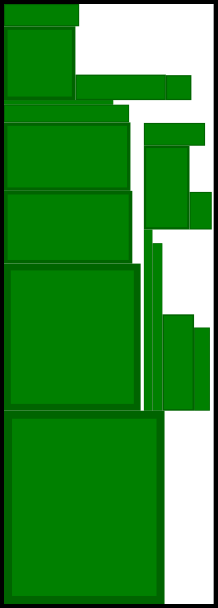
\includegraphics[width=.5\linewidth]{SplitFitrun.png}
  \caption{Split-Fit Algorithm}
  \label{fig:splitfitrun}
\end{subfigure}
  \caption{Visualisation of FFDH and SF for the same problem instance. The packing of $L_2$ objects into the Split-Fit rectangle $R$ can be seen in \ref{fig:splitfitrun}.}
  \label{fig:ffdhsfrun}
\end{figure}


\section{Brute Force Algorithm}
We describe an optimal solution for 2-D Strip Packing. The algorithm is based off the Maximal Rectangles (MAXRECT) algorithm \cite{maxrects}. We begin with a simple result:

\begin{defn}
For any feasible packing of a subset of objects, we call the packing tight if every object cannot be moved leftwards or downwards an infinitesimal amount. (i.e. it is touching another object or a boundary on both its left and bottom sides)
\end{defn}

\begin{thm}
There exists an optimal solution which is tight.
\end{thm}
This is clear as from any optimal solution, we can always move any object leftwards or downwards without increasing the total height, until no object can be moved leftwards or downwards any further.\\

In the MAXRECT algorithm, we place each object sequentially, to construct a feasible solution, while maintaining that the current placement is tight at each step. When we have placed all rectangles, the total height of the rectangles is noted. An exhaustive search of all tight packings is done, to find the tight packing of minimum height.

\begin{defn}
A Free Rectangle is defined as any rectangle that covers open space. (i.e. it does not intersect any existing object)
\end{defn}

\begin{defn}
A Maximal Free Rectangle (Maximal Rectangle) is a Free Rectangle that is not a subset of any other Free Rectangle.
\end{defn}

To do this, we maintain a list of Maximal Rectangles that represent the possible positions one can place the next object. Each Maximal Rectangle represents an area of open space where objects can be placed. By theorem \ref{thm:blmaxrect} each possible object placement position corresponds to placing the object at the bottom left of some maximal rectangle. This also shows that we are able to construct any tight packing using this method.

\begin{thm}
\label{thm:blmaxrect}
When add a new object $s$ to a currently tight packing $P$, if the new packing is tight, then $s$ is at the bottom left corner of some maximal rectangle in packing $P$.
\end{thm}
\begin{proof}
If the new packing is tight, the new object cannot be moved leftwards or downwards. We can thus construct a free rectangle covering the object exactly. The free rectangle cannot be extended leftwards or downwards as the original object was obstructed in those directions. We can thus extend the width rightwards, then height upwards to the maximum possible to make it maximal.
\end{proof}

We note that to maintain the tightness property of the packing, we will need to additionally check that there newly placed object is touching another object (or boundary) on both its bottom and left sides. If the new object fails this check, we do not consider this possible placement. For example, in Figure \ref{fig:floatingmaxrect}, the new packing is no longer tight, even though the new object has been placed in the bottom left corner of a maximal free rectangle.

\begin{figure}[!h]
  \centering
  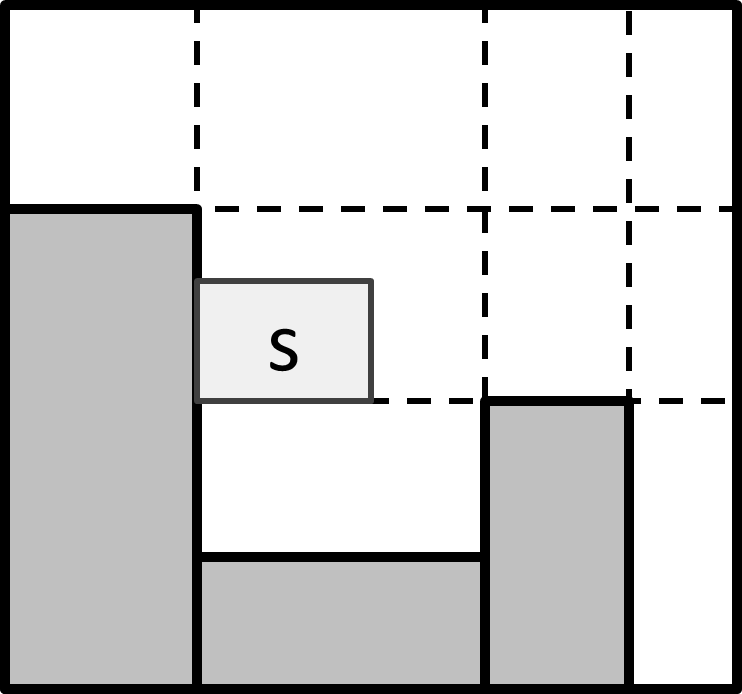
\includegraphics[width=.4\linewidth]{diagrams/floatingmaxrect.png}
  \caption{The object $s$ is placed at the bottom left corner of a maximal rectangle, but the new packing is not tight.}
  \label{fig:floatingmaxrect}
\end{figure}

We now explain how we can maintain the list of Maximal Rectangles. At the beginning of the algorithm with an empty packing (no objects), there is exactly one maximal rectangle, which consists of the whole strip. (a free rectangle is allowed to have a height of $\infty$). Whenever a new object is placed, the new object is checked for intersection with each existing maximal rectangle in the list. For each maximal rectangle the object intersects, the maximal rectangle is split into multiple maximal rectangles, as detailed by the 16 cases in figure \ref{fig:maxrectsplitting}. (Note: three of the cases cannot occur.)

\begin{figure}[!h]
  \centering
  \begin{subfigure}{.25\textwidth}
    \centering
    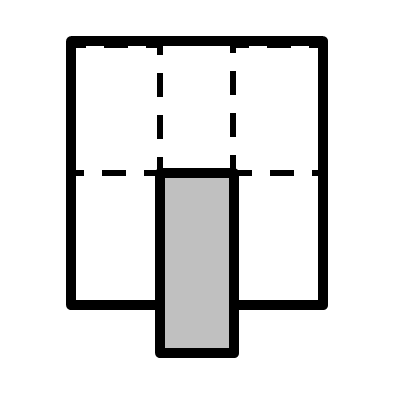
\includegraphics[width=.95\linewidth]{16cases/c1.png}
    \caption{}
    \label{fig:c1}
  \end{subfigure}%
  \begin{subfigure}{.25\textwidth}
    \centering
    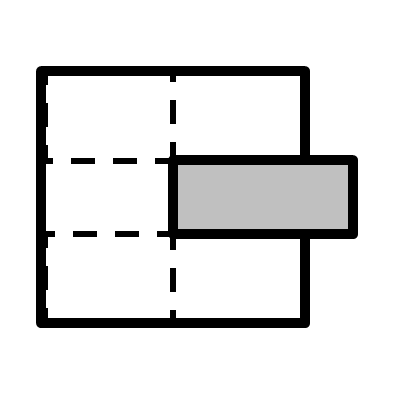
\includegraphics[width=.95\linewidth]{16cases/c2.png}
    \caption{}
    \label{fig:c2}
  \end{subfigure}%
  \begin{subfigure}{.25\textwidth}
    \centering
    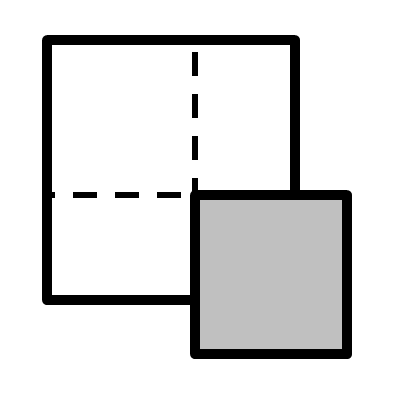
\includegraphics[width=.95\linewidth]{16cases/c3.png}
    \caption{}
    \label{fig:c3}
  \end{subfigure}%
  \begin{subfigure}{.25\textwidth}
    \centering
    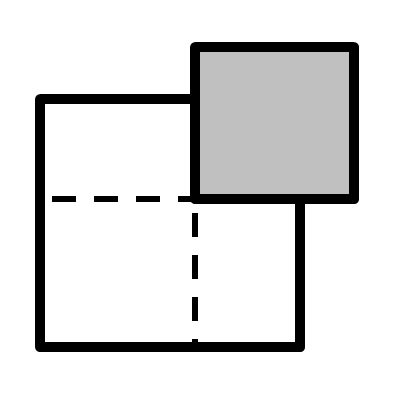
\includegraphics[width=.95\linewidth]{16cases/c4.png}
    \caption{}
    \label{fig:c4}
  \end{subfigure}\\
  \begin{subfigure}{.25\textwidth}
    \centering
    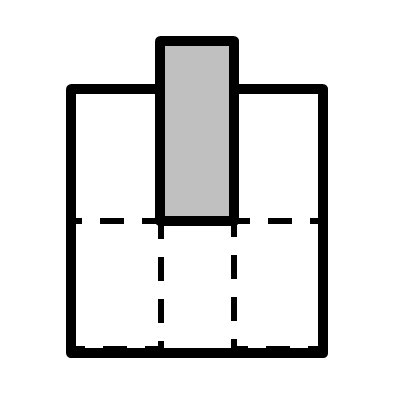
\includegraphics[width=.95\linewidth]{16cases/c5.png}
    \caption{}
    \label{fig:c5}
  \end{subfigure}%
  \begin{subfigure}{.25\textwidth}
    \centering
    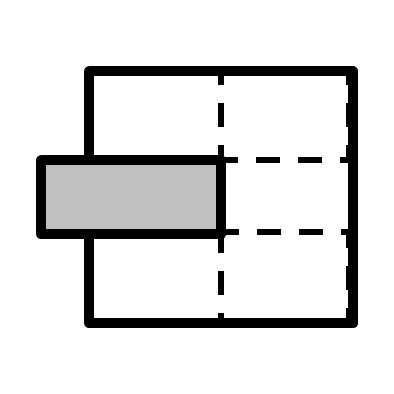
\includegraphics[width=.95\linewidth]{16cases/c6.png}
    \caption{}
    \label{fig:c6}
  \end{subfigure}%
  \begin{subfigure}{.25\textwidth}
    \centering
    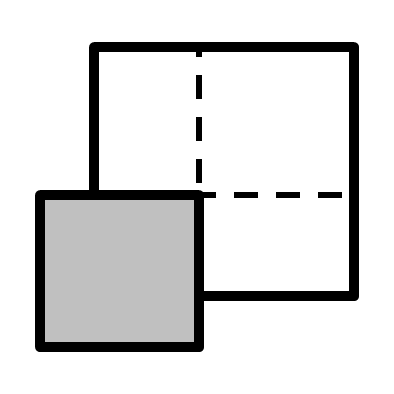
\includegraphics[width=.95\linewidth]{16cases/c7.png}
    \caption{}
    \label{fig:c7}
  \end{subfigure}%
  \begin{subfigure}{.25\textwidth}
    \centering
    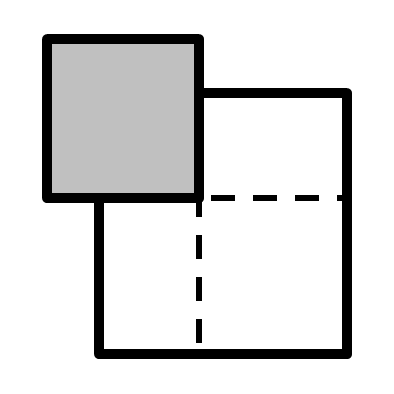
\includegraphics[width=.95\linewidth]{16cases/c8.png}
    \caption{}
    \label{fig:c8}
  \end{subfigure}\\
  \begin{subfigure}{.25\textwidth}
    \centering
    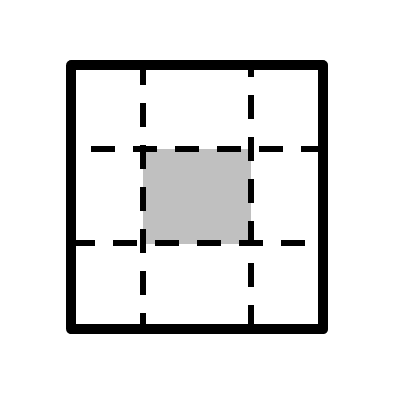
\includegraphics[width=.95\linewidth]{16cases/c9.png}
    \caption{}
    \label{fig:c9}
  \end{subfigure}%
  \begin{subfigure}{.25\textwidth}
    \centering
    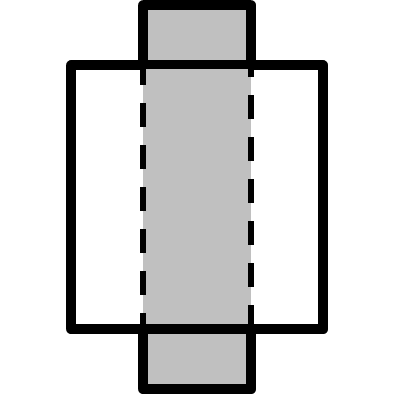
\includegraphics[width=.95\linewidth]{16cases/c10.png}
    \caption{}
    \label{fig:c10}
  \end{subfigure}%
  \begin{subfigure}{.25\textwidth}
    \centering
    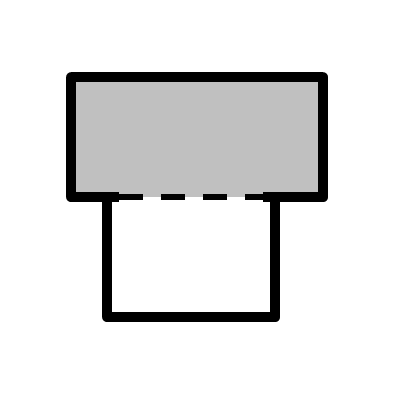
\includegraphics[width=.95\linewidth]{16cases/c11.png}
    \caption{}
    \label{fig:c11}
  \end{subfigure}%
  \begin{subfigure}{.25\textwidth}
    \centering
    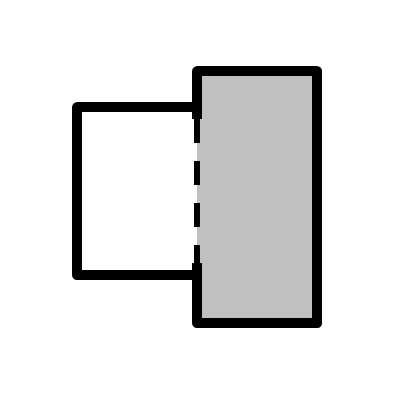
\includegraphics[width=.95\linewidth]{16cases/c12.png}
    \caption{}
    \label{fig:c12}
  \end{subfigure}\\
  \begin{subfigure}{.25\textwidth}
    \centering
    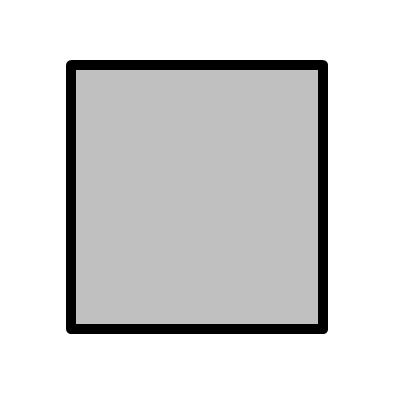
\includegraphics[width=.95\linewidth]{16cases/c13.png}
    \caption{}
    \label{fig:c13}
  \end{subfigure}%
  \begin{subfigure}{.25\textwidth}
    \centering
    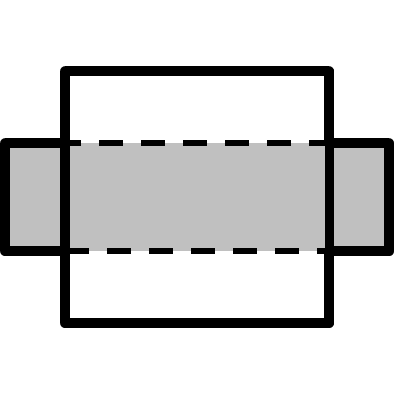
\includegraphics[width=.95\linewidth]{16cases/c14.png}
    \caption{}
    \label{fig:c14}
  \end{subfigure}%
  \begin{subfigure}{.25\textwidth}
    \centering
    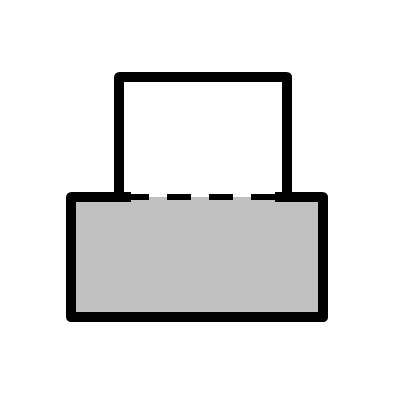
\includegraphics[width=.95\linewidth]{16cases/c15.png}
    \caption{}
    \label{fig:c15}
  \end{subfigure}%
  \begin{subfigure}{.25\textwidth}
    \centering
    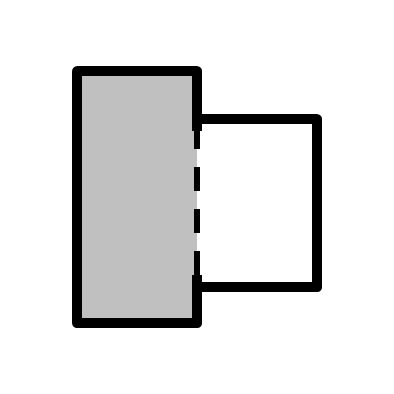
\includegraphics[width=.95\linewidth]{16cases/c16.png}
    \caption{}
    \label{fig:c16}
  \end{subfigure}%
  \caption{The 16 cases for splitting maximal rectangles.}
  \label{fig:maxrectsplitting}
\end{figure}

\begin{thm}
\label{thm:maxrectgeneration}
When placing a new object, every new maximal rectangle generated is a subset of some maximal rectangle in the packing before placing the new object.
\end{thm}
\begin{proof}
Consider any new maximal rectangle $r$ in the new packing. When the newly placed object is removed to obtain the previous packing, $r$ is still a free rectangle in the old packing, meaning it is the subset of some maximal rectangle.
\end{proof}

Theorem \ref{thm:maxrectgeneration} shows that the splitting of maximal rectangles will exhaustively identify all new maximal rectangles. However, we note that not all rectangles generated by splitting will be maximal (Figure \ref{fig:splitbutnotmaxrect}). To check that a rectangle is not maximal, we need to check whether there is an obstruction on each of the sides of the free rectangle that prevents the free rectangle from being expanded further.

\begin{figure}[!h]
  \centering
  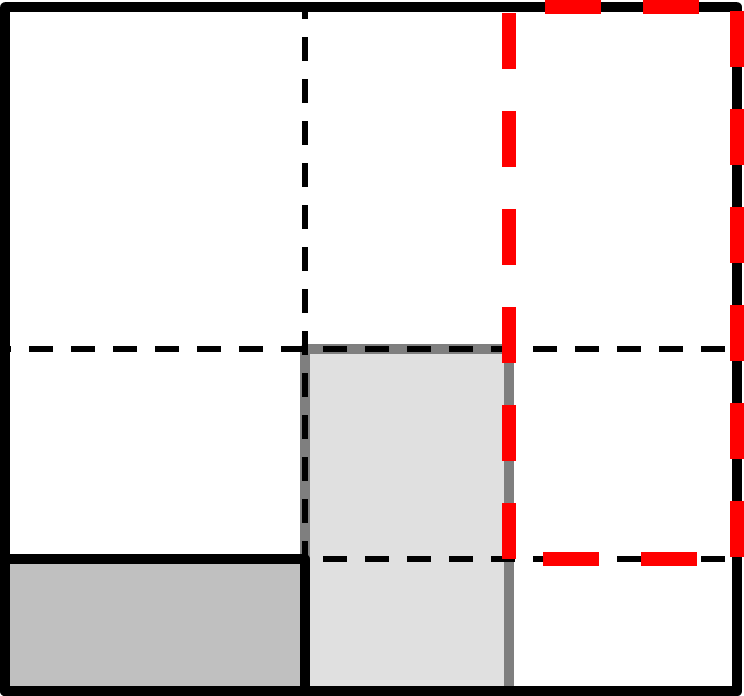
\includegraphics[width=.4\linewidth]{diagrams/splitbutnotmaxrect.png}
  \caption{A free rectangle resulting from a split that is not a maximal rectangle.}
  \label{fig:splitbutnotmaxrect}
\end{figure}

For efficient checking for the existence of an obstruction, we define the notion of a support as follows:

\begin{defn}
In a packing $P$, The top/bottom/left/right support of a free rectangle is defined as the set of placed objects directly touching the top/bottom/left/right edges of the free rectangle respectively. Objects touching the free rectangles only at the corners do not count as part of the support.
\end{defn}

Thus, a free rectangle is maximal if and only if for each of its four sides, it has either a nonempty support or is touching the boundary of the strip at that side. From theorem \ref{thm:supportinheritance}, we only need to check the support of the parent rectangle (Definition \ref{defn:parentrectangle}) and the most recently placed object to generate the support of the new free rectangle. If the support on any of the sides is empty, we prune the free rectangle if any only if the support of the parent rectangle on the same side is not empty. (We note that if the support of the parent rectangle on that side is empty, that side must be touching the boundary of the strip as the parent rectangle has not been pruned).

\begin{defn}
\label{defn:parentrectangle}
When a maximal rectangle is split to form free rectangles, the parent rectangle of the newly-formed free rectangles is the maximal rectangle it was split from.
\end{defn}

\begin{thm}
\label{thm:supportinheritance}
When a free rectangle $r$ is split from placing an object $s$ into a maximal rectangle $p$ (the parent rectangle), on each side $T$, the support of $r$ on side $T$ is either $\{s\}$ or a subset of the support of $p$ on side $T$.
\end{thm}
\begin{proof}
This is easy to see, as for each of the cases shown in figure \ref{fig:maxrectsplitting}, each of the newly created free rectangles share three sides with the parent rectangle $p$, and the last side touches the object $s$. The side touching the object $s$ has only $s$ as its support, and the other three sides' supports are subsets of the respective sides' support in the parent rectangle $p$.
\end{proof}

There are two other cases we need to consider for maintaining the support lists of each maximal rectangle correctly. Firstly, for the maximal rectangle created at the start of the algorithm, we can initialise each of its support lists to be empty, as it is touching all four of the boundaries of the strip. Secondly, if a newly-placed object happens to be touching an existing maximal rectangle at a boundary, we need to add the newly-placed object to the support of the maximal rectangle. This check can be done at the same time as when we are checking whether the newly placed object intersects any maximal rectangles.\\

Thus, through this method, we are able to maintain a list of the maximal rectangles at any point of the algorithm. At each node in the search tree, for each unplaced object and for each maximal rectangle, if we can place the object into the maximal rectangle (the object's dimensions fits into the boundaries of the maximal rectangle), we try placing that object into that maximal rectangle. Thus, we have created a brute-force algorithm that searches through all possible tight packings, and thus will be able to find an optimal solution for the 2-D Strip Packing problem.

\subsection{Asymptotic Analysis of Running Time}
We let the number of rectangles to be fitted by $n$.\\
We note that the number of maximal rectangles at any point of time is at most $3k$, where $k$ is the number of already placed objects. The number of unplaced objects at this point of time is $n-k$. The branching factor at recursion depth $k$ is thus $3k(n-k)$.\\

At each node, when placing a new rectangle $r$ at recursion depth $k$, we have to check its intersection with each of the $\leq 3k$ maximal rectangles. For each maximal rectangle $k$ that has been split, checking and copying over the support takes $O(k)$ time per rectangle. Thus we have a running time of $O(k^2)$ per node.\\

This makes a total running time of $\displaystyle\sum_{m=0}^{n-1} (\prod_{k=1}^{m} 3(k)(n-k))(k-1)^2$. As the last term of this sum dwarfs the sum of the first $n-1$ terms asymptotically, the running time is $O((\prod_{k=1}^{n-1} 3(k)(n-k))(k-1)^2) = O(3^n(n-1)!(n-1)!(n-1)^2) = O(3^n(n!)^2)$.

\subsection{Pruning Rules}

\subsubsection{Branch and Bound} \label{sssec:branchandbound}
The most basic pruning rules are the upper bound and lower bound pruning rules of branch and bound. At all times, we maintain an upper-bound value $U$. We initialise $U$ to a known upper bound (for example, the sum of the heights of the rectangles, or the solution found by a heuristic algorithm like FFDH). Whenever we find a feasible solution of total height less than $U$, we update the value of $U$ to the height of the solution found. Now, at any point of the algorithm, if the current total height of the placement $P$, $height(P) \geq U$, we can prune the current branch.\\

At any point of the algorithm, let $S$ be any subset of the remaining unplaced objects. Suppose that we can find a lower bound $L(S)$ for the minimum-height strip that can pack all of the objects in $S$. Let $h$ be the height of the lowest maximal rectangle that can fit some element in $S$. We can then prune the current branch if $L(S) + h \geq U$.

Here are some ways in which these rules can be used:
\begin{enumerate}
\item Let $S$ be the set containing only the rectangle of maximum height. The lower bound $L(S)$ would thus be the height of $S$.

\item Let $S$ be the set of all "wide" objects (objects with width stictly greater than half the width of the strip). As these objects can only be stacked directly on top of each other, the lower bound for $S$ would be the sum of the heights of the objects in $S$.

\item Let $S$ be any subset of the remaining set (preferably the wider rectangles). We run the FFDH algorithm on only these rectangles, which has an approximation ratio of $1.7OPT + 1$. Suppose the FFDH algorithm returns a height of $T$. Thus we can obtain a lower bound for $S$ as $L(S) = \frac{T - 1}{1.7}$.
\end{enumerate}

As the third rule is unpromising due to $\frac{T-1}{1.7}$ not being a useful lower bound in most cases due to is low, and sometimes negative value, we only make use of rules 1 and 2 for our lower bound checks.


\subsubsection{Symmetry Removal}
As we are allowed to place the rectangles in any order, a common problem that occurs during our rectangle placement is repeat computations. For example, in figure \ref{fig:repeatplacements}, the rectangles $a,b,c,d$ can be placed in $4!$ possible orders, each corresponding to a different branch. As each of these packings are equivalent, only one of the packings need to be explored.\\ 

\begin{figure}[!h]
  \centering
  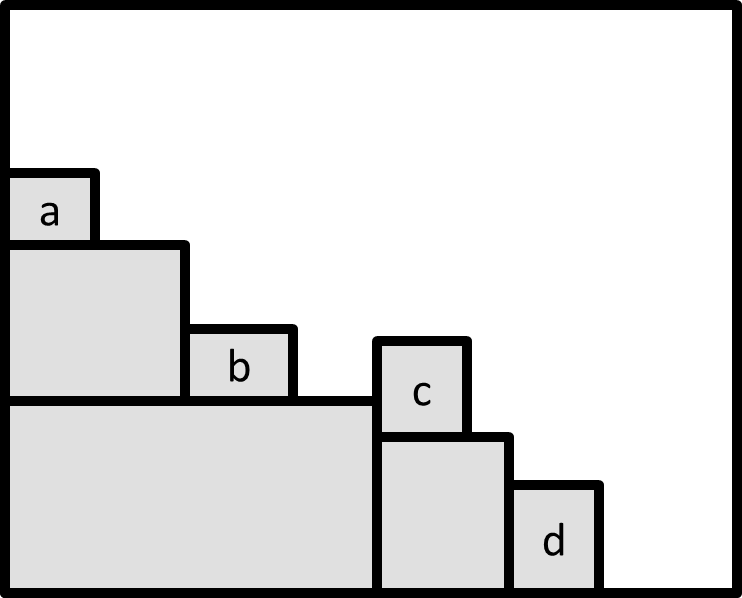
\includegraphics[width=.4\linewidth]{diagrams/repeatplacements.png}
  \caption{This packing can be built from many possible placement orders}
  \label{fig:repeatplacements}
\end{figure}

A simple way of preventing repeated computations is by storing information on which computations have been done before. However, due to the large amount of branches, this will require an exponential amount of memory to store. Theorem \ref{thm:fixedordering} provides an alternative way of pruning symmetric branches without storing any additional memory.

\begin{thm} Fixed Ordering\\
\label{thm:fixedordering}
Suppose that we have a function $f$ that takes in a packing $P$, that returns an order in which the objects can be placed for form $P$, with the following properties:
  \begin{enumerate}
  \item $f$ is well defined - it deterministically produces an ordering from only the current positions of the objects.
  \item Take any placement $P$ with some $m \in \mathbb{N}$ placed rectangles. For each $k \in \{1,\cdots,m\}$, the packing $P_k$ consisting only of the first $k$ placed rectangles in $f(P)$ is tight, and $f(P_k)$ assigns the same orders to the $k$ rectangles as $f(P)$.
  \end{enumerate}
And suppose we add the pruning rule: Suppose the current packing is $P$. If the order in which the rectangles were placed is not equal to $f(P)$, then prune the branch.
Then we will have the following:
  \begin{enumerate}
  \item For every feasible placement $P$, $P$ can be constructed by some possible placement order by the algorithm with the pruning rule.
  \item For every feasible placement $P$, there is exactly one placement order in which $P$ can be constructed.
  \end{enumerate}
\end{thm}
\begin{proof}~\\
\begin{enumerate}
\item
This is clear as the items can be placed in the order $f(P)$ to construct the placement $P$ by the second property of the function $f$.
\item
This is also clear as $P$ cannot be constructed in any order other than $f(P)$.
\end{enumerate}
\end{proof}

Thus, by properly defining an "ordering function" $f$, we will be able to create a pruning rule that ensures that each packing $P$ is explored no more than once. We thus define a function $f$ in the following manner:\\

Take a tight packing $P$. Let $s_1,s_2,\cdots,s_m$ be the ordering of the $m$ placed objects given by $f(P)$. To define $s_k$, we consider the placement of $s_1,\cdots,s_{k-1}$. Out of all the remaining objects that can be "placed" while maintaining a tight packing, let $s_k$ be the one with minimum $y$. If there are ties, we pick the one with lowest $x$ value. Note that we compare the bottom left corners of the objects. By this construction, we ensure that property 2 will be satisfied by function $f$.

\subsubsection{Early Discovery of Lower Bounds}
We can derive an additional lower-bound pruning rule using the following theorem:

\begin{thm}
\label{thm:kprune}
Let $P$ be the current packing and $S$ be a subset of the remaining unpacked objects. Suppose that any tight placement of rectangles in $S$ into $P$ has height at least $U$. Then there is no placement of the remaining unpacked objects onto $P$ with height less than $U$.
\end{thm}
\begin{proof}
This is clear as from any packing of the remaining objects with height less than $U$, all remaining objects not in $S$ can be removed, and the objects in $S$ can be shifted left and down to make a tight packing with height less than $U$.
\end{proof}

Thus, we use the following search order: we iterate through the objects in a fixed order (e.g. by index). For each object, we try to fit it into each of the maximal rectangles, before moving on to the next unplaced rectangle.\\

This way, we can apply the following pruning rule:\\
Consider the current search node (corresponding to some packing $P$) with $m$ remaining unplaced objects $\{s_1,s_2,\cdots,s_m\}$, that will be fitted in the order $s_1,s_2,\cdots,s_m$. For any $k \in \{1,\cdots,m-1\}$, if trying to place the objects $s_1,\cdots,s_k$ each produces a recursion depth of at most $k$, we can prune the current node without attempting to place the objects $s_{k+1}$ onwards.\\

This works because from the fixed order of placing objects, as the recursion depths are at most $k$, all possible combinations of trying to place objects $s_1,s_2,\cdots,s_k$ must have failed, meaning that it is impossible to place $s_1,\cdots,s_k$ onto packing $P$ without the remaining height being at least the upper bound $U$. Note, however, that this pruning rule does not work with existing pruning rules, as this rule assumes that pruning only occurs when the current total height is at least the upper bound $U$.\\

\begin{figure}[!h]
  \centering
  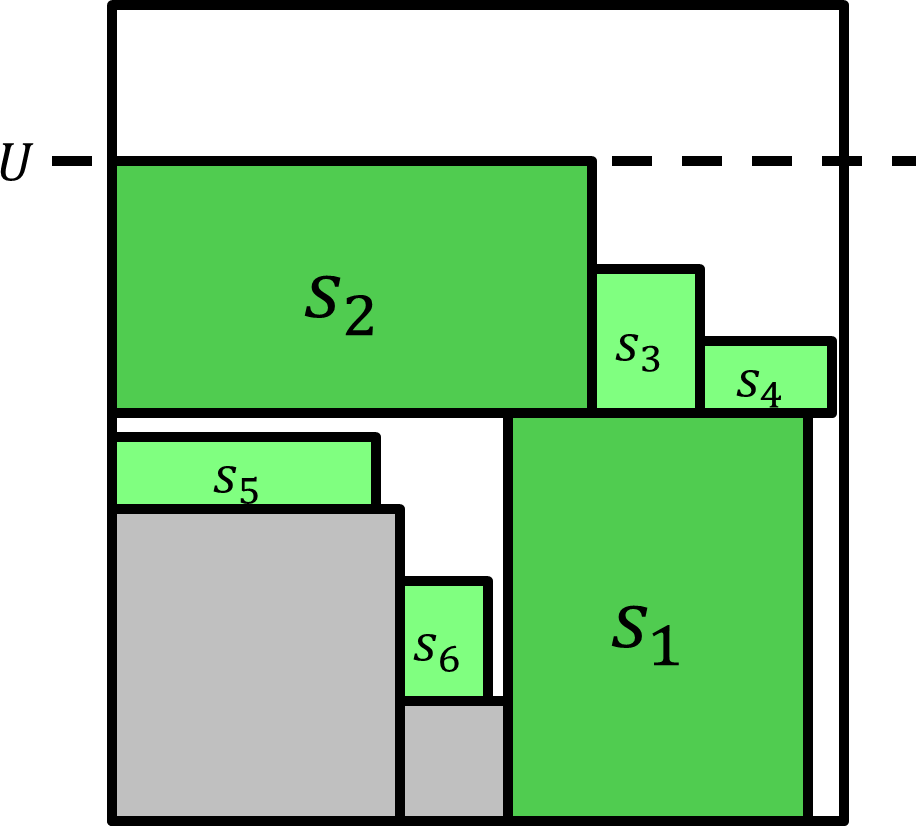
\includegraphics[width=.4\linewidth]{diagrams/earlylowerbounds.png}
  \caption{An example where the early lower-bound pruning rule is effective.}
  \label{fig:earlylowerbounds}
\end{figure}

An example where this rule is effective is in figure \ref{fig:earlylowerbounds}. In the figure, the gray rectangles are the current placement $P$, and the green rectangles $s_1,\cdots,s_6$ are the yet unplaced rectangles. We place the rectangles in the order $s_1,s_2,s_3,s_4,s_5,s_6$. We note that the algorithm will first try placing $s_1$, then $s_2$, fail as it exceeds the upper bound $U$, then try placing $s_2$, then $s_1,$ and fail as it once again exceeds the upper bound $U$. At this point, we can already deduce that it is impossible to fit $s_1$ and $s_2$ into the current formation without the total height being at least $U$. The rule would thus prune at this point with $k = 2$.\\

Without the rule, the algorithm would then proceed to try placing $s_3$ first, then $s_4$ first, and so on, continuing for a very long time before actually pruning this node.

\section{Experimental Results}
For problems of relatively small size (20 objects and below), our implementation of the branch-and-bound algorithm finds the optimal solution within a reasonable amount of time. For the 20-object case, the branch-and-bound algorithm completes after approximately 10 minutes on a Lenovo ThinkPad x230 running a 2.60 Ghz Intel i5 processor.\footnote{This machine was also used to carry out the rest of the experiments.} For our experiments, we consider cases below 20 objects as small instances, and cases with more than 20 rectangles as large instances.

\subsection{Small instances}
For small instances, we can use the branch-and-bound algorithm to find the optimal solution. As mentioned at the beginning of section \ref{sssec:branchandbound}, we can choose to generate an initial upper-bound $U$ with a heuristic like FFDH to prune the initial branches the search. For our implementation, the branch-and-bound algorithm would run \textit{both} FFDH and Split-Fit and use the better solution as the upper bound.\\
\\
Furthermore, we observed that the running time behind the branch-and-bound algorithm is very dependent on the order in which we sort (and thus, explore) the objects. Leaving the objects in their original, randomized order is almost always worse than working with a set of objects pre-sorted by decreasing height or decreasing width. However, we found the algorithm worked best when the objects are pre-sorted by their areas.\\
\\
We believe that this is because the large area of the initial rectangles provides less room for other rectangles to fit in, and thus they can either improve the currently optimal value, or be pruned early by either a \textit{best-solution-so-far} upper bound or the lower bound found by Theorem \ref{thm:kprune}. Thus, we would reach better heights, and thus be able to prune cases, faster.\\
\\
For small instances, shortened instances from Zhang et al.'s dataset are used (the complete instances from this dataset are used as large instances in the next section). Table \ref{table:smallinstances} compares the running time of the branch-and-bound algorithm with objects sorted in different orders for various small instances.

\begin{table}
\centering
\begin{tabular}{|c|c|c|c|c|c|}
\hline Name & Items & Width & Decreasing Height & Decreasing Width & Decreasing Area \\
\hline zdf1 & 580 & 100 & 402 & 402 & 1 \\
\hline zdf2 & 660 & 100 & 428 & 431 & 1\\
\hline
\end{tabular}
\caption{Running time (in seconds) of branch-and-bound algorithm with exploration orders}
\label{table:smallinstances}
\end{table}

\subsection{Large instances}
To test the effectiveness of the FFDH and Split-Fit heuristic algorithms, we run them on large datasets. The dataset used is Zhang et al.'s ZDF dataset, which is generated by combining zero-waste and nonzero-waste data \cite{zdf}. We find that, even though Split-Fit has a slightly better asymptotic approximation ratio than FFDH, it does worse than FFDH in most of the test cases given Table \ref{table:zdftest}.

\begin{table}
\centering
\begin{tabular}{|c|c|c|c|c|}
\hline Name & Items & Width & FFDH Height & SF Height \\
\hline zdf1 & 580 & 100 & 402 & 402 \\
\hline zdf2 & 660 & 100 & 428 & 431 \\
\hline zdf3 & 740 & 100 & 453 & 458 \\
\hline zdf4 & 820 & 100 & 477 & 481 \\
\hline zdf5 & 900 & 100 & 503 & 506 \\
\hline zdf6 & 1532 & 3000 & 5583 & 5608 \\
\hline zdf7 & 2432 & 3000 & 5567 & 5608 \\
\hline zdf8 & 2532 & 3000 & 5867 & 5877 \\
\hline zdf9 & 5032 & 3000 & 5861 & 5885 \\
\hline zdf10 & 5064 & 6000 & 5726 & 6264 \\
\hline zdf11 & 7564 & 6000 & 5728 & 6251 \\
\hline zdf12 & 10064 & 6000 & 5720 & 6259 \\
\hline zdf13 & 15096 & 9000 & 5718 & 5912 \\
\hline zdf14 & 25032 & 3000 & 5875 & 5898 \\
\hline zdf15 & 50032 & 3000 & 5882 & 5901 \\
\hline zdf16 & 75032 & 3000 & 5881 & 5903 \\
\hline
\end{tabular}
\caption{FFDH and Split-Fit's performance on Zhang et al.'s dataset.}
\label{table:zdftest}
\end{table}

\section{Conclusion}
Seth is handsome

\begin{thebibliography}{9}
\bibitem{harren1}
  Harren, R., Jansen, K., Pradel, L., van Stee, R.:
  \emph{A (5/3 + $\epsilon$)-Approximation for Strip Packing},
  In: WADS 2011 : Algorithms and Data Structures Symposium

\bibitem{baker1}
  Baker, B.S., Brown, D.J., Katseff, H.P.:
  \emph{A 5/4 algorithm for two-dimensional packing},
  Journal of Algorithms 2(4) (1981) 348–368

\bibitem{maxrects}
  Jukka Jylanki:
  \emph{A Thousand Ways to Pack the Bin - A Pratical Approach to Two-Dimensional Rectangle Bin Packing},
  retrived from http://clb.demon.fi/files/RectangleBinPack.pdf, 2010

\bibitem{zdf}
  Zhang, D., Wei, L., Leung, S.C.H., Chen, Q.,
  \emph{A Binary Search Heuristic Algorithm Based on Randomized Local Search for the Rectangular Strip Packing Problem},
  INFORMS Journal on Computing 25 (2) (2013) 332-345
\end{thebibliography}

\end{document}